% !TEX root = C:/Users/piyus/knowledge/EE/yang_lab/papers/The BrainScaleS-2 Accelerated Neuromorphic System With Hybrid Plasticity/notes.tex
\documentclass[12pt, letterpaper]{article}

\usepackage{graphicx}
\graphicspath{ {C:/Users/piyus/knowledge/EE/yang_lab/papers/The BrainScaleS-2 Accelerated Neuromorphic System With Hybrid Plasticity/pictures} }

\title{Notes on "The BrainScaleS-2 Accelerated Neuromorphic System With Hybrid Plasticity"}
\author{Piyush Sud}
\date{8/22/2024}
\begin{document}
\maketitle

\pagebreak

\section{Abstract}
\begin{itemize}
    \item This paper describes the BrainScaleS SNN, which has both analog and digital components.
\end{itemize}


\section{Introduction}
\begin{itemize}
    \item BrainScaleS provides continuous time modeling of the brain using a physical replica of neurons connected with synapses.
    \item BrainScaleS uses CMOS instead of nano-devices for this continuous modeling to create configurable behavior.
    \item This system addresses the time and temperature drift problem of most analog systems.
    \item On chip calibration is acheived with embedded processors and ADCs.
    \item This chip can be operated in many different modes - the first is batch mode, where there are no data dependencies between experiments.
    \item This chip supports fine control of synaptic plasticity.
    \item Analog data is acquired in parallel, while the plasticity changes are computed efficiently using a digital processor.
    \item Vector matrix multiplication can be realized for ANNs. 
\end{itemize}

\section{The BrainScaleS-2 System}
\subsection*{System Architecture}
\begin{itemize}
    \item The system designed so far can be considered as a single core, which can theoretically be used as a building block for a large SNN.
    \item A single core consists of:
    \begin{itemize}
        \item 4 256x128 synaptic crossbars, each containing 128 neurons, with one neuron corresponding to a single column.
        \item Two digital processors for controlling the plasticity of the synapses.
        \item Two 512 channel ADCs. Each quadrant has 256 channels, since 128 channels are used for spike train correlation measurements and the other 128 channels are used for spike train anti-correlation measurements.
        \item Analog parameter storage
        \item An event routing network for spike communication. The outputs of the neurons can either be routed back to the inputs or to an external output.
    \end{itemize}
    \item This chip has been used in two hardware setups, one for analog measurements and the other for edge devices, with a Zynq FPGA SoC.
    \item In the future, an external event routing network could be used with 8 cores on a single chip.
\end{itemize}

\subsection*{Accelerated Analog Emulation of Neural Dynamics}
\begin{itemize}
    \item The speed of the semiconductors is around 1000x the speed of biological neural networks in order to work with the time constants of semiconductor materials.
    \item The neurons are implemented using mixed-signal circuits (it's unspecified what the exact circuit is), which follow the adaptive exponential integrate-and-fire (ADEX) model.
    \item The first equation says that C\(\frac{dV}{dt}\)\ = the leakage current into the extracellular fluid + the current caused by positive feedback of Na+ ions - the adaptation/refractory current after a spike + the current I flowing into the membrane through external stimuli, where C is the capacitance of the membrane and V is the membrane potential. E1 is the resting potential of the extracellular fluid.
    \item 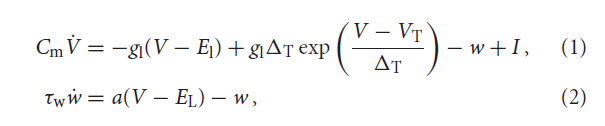
\includegraphics{ADEX.png}
    \item The second equation describes the adaptation current after a spike has been fired, which decays to 0 with time constant tw.
    \item Each neuron can be configured with 80 bits of SRAM and 24 analog paramters which are set by a 10-bit DAC. Since each neuron can be controlled individually, production deviations can be compensated for to create an ideal network. Parameters such as the refractory period and membrane capacitance can be programmed.
    \item Each neuron integrates the current from all 256 synapses.
    \item The following equation describes the current flowing into a neuron, and is equal to the weighted sum of the spike trains multiplied by an exponential decay.
    \item 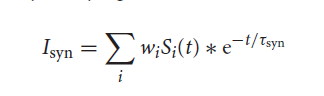
\includegraphics{synapse_current.png} 
    \item The weights are stored locally per synapse in a 6-bit SRAM.
    \item Instead of using muxes to route synapses, a 6-bit address is associated with each synapse. If there is a connection between the output of a neuron and a synapse, then any "event packets" that are sent on the output of that neuron will contain the address of the synapse, which will check for a matching address and respond only if the address matches.
    \item Analog sensor circuits on each synapse can be used to accurately measure the spike timing, which in turn can be used for STDP.
    \item By disabling the spiking behavior, a regular non-time continuous VMM can be performed.
\end{itemize}

\subsection*{Hybrid Plasticity and Versatile Digital Control}
\begin{itemize}
    \item The PPU (Plasticity Processing Unit) is designed to be very flexible to allow for many different digital configurations.
    \item The ASIC can perform tens of thousands of correlation measurements per second.
    \item The plasticity programs can perform both fixed point and integer computations on either a 128 x 8 bit or 64 x 16 bit vector.
    \item This has been used to demonstrate several versions of STDP. 
    \item Out-of-order-execution is used to speed up the plasticity computations, which allows for vector computations and scalar computations to occur simultaneously.
    \item The parallel access to the neuron outputs with the column ADC allows for efficient on-chip calibration.
    \item The 32-bit POWER ISA is used with a compiler and the C++ programming language.
    \item The SIMD (Single Instruction, Multiple Data) vector instructions are custom but very similar to the POWER ISA ones.
    \item They modified the GCC compiler to work with their modified ISA and added support for the C++ standard library.
    \item While on-chip memory is limited to 16 KiB per processor core, they have access to an external memory interface, which is higher latency but larger in size.
\end{itemize}

\section*{Applications of the BrainScaleS-2 System}

\subsection*{Faithful Emulation of Complex Dynamics}

\begin{itemize}
    \item The BrainScaleS system allows for detailed control of each circuit and in turn each model parameter.
    \item The on-chip ADC is 10-bits and operates at a frequency of 29 MHz.
    \item A FPGA reads and buffers the ADC data, and also handles experiment control.
    \item For each firing pattern, the neurons were stimulated with a current pulse of width 350 us, and they measured the adaptation voltage (from which current can be estimated) and the membrane potential.
    \item Four different spiking patterns were observed by varying different parameter such as the adaptation strength a and adaptation increments b.
    \item 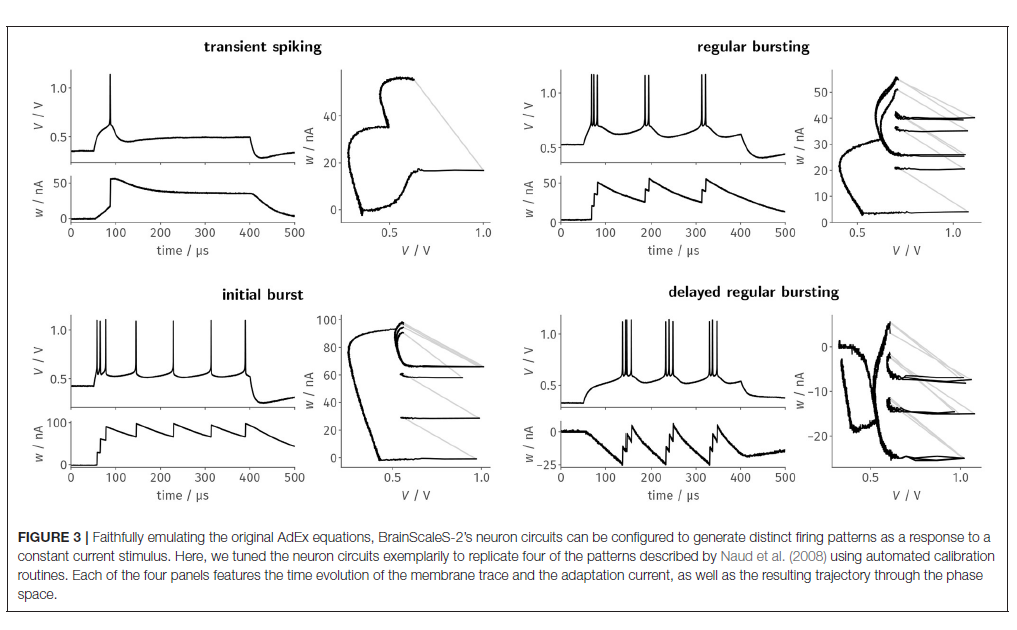
\includegraphics{spike_patterns.png}
    \item As shown in the graphs of V vs. w, the neuron spiking is very reproducible and the number of spikes for the same stimulus is almost exactly the same for all 128 neurons.
    \item The BrainScaleS-2 system also supports multi-compartment models, where the neurons are grouped together into 4 compartments, and the output of one compartment is connected to the input of the next.
    \item A synaptic input was injected to a different compartment each experiment, and as expected, that input traveled to the compartments following it, but was slightly attenutated with each compartment.
    \item Plateau potentials are also acheived in compartments by modifying some neuron parameters and providing two inputs (one being delayed) in order to trigger a plateau. A plateau was triggered when the latter compartment spikes before the former, and the time between the spikes at a synapse is inversely proportional to the likelihood of a plateau occuring.
\end{itemize}

\subsection*{Biology Inspired Learning Approaches}

\begin{itemize}
    \item In order for a learning rule to be biologically plausible, it has to be spatially and temporally local. Spatially local means that neurons can only observe what is directly connected to them. By temporally local, it means that the neuron can make a calculation in a very short time period in response to a stimuli, without seeing the global behavior.
    \item Multiple reinforcement learning rules were realized on the platform, including playing pong and maze navigation.
    \item Other biological behavior includes the possibility of synaptic pruning and rewiring and sparse connectivity.
    \item Inspect inspired navigation is also demonstrated. The spiking neural network is configured to represent a bee brain, and the bee hunts for food and returns to its nest. The system runs at 1000x real time. The environment of the bee is simulated using on the on-chip processor in the PPU. 
    \item Since the system is accelerated, tuning hyperparameters takes a very small amount of time.
    \item The host computer implemented the evolutionary algorithm to allow the bee to learn.
    \item The system was also used for closed-loop robotics. Since the neuron dynamics are very accelerated, the robotic system had to be on microsecond time scale.
\end{itemize}


\end{document}